\documentclass{article}

\usepackage{amsmath}
\usepackage{graphicx}
\usepackage{hyperref}
\usepackage[utf8]{inputenc}
\usepackage{minted}

\title{Simple 3D engine med pygame}

\author{Christian Linde Ahrnkiel\\
Synopsis Prog B eksamensprojekt\\
Odense Tekniske Gymnasium
}

\date{9. Maj 2025}

\begin{document}

\maketitle
\tableofcontents

\newpage
\section{Indledning}
\subsection{Formål}
Formålet med dette projekt er at lave en simple 3D engine.
En 3D engine er et program der kan vise 3D objekter på en 2D skærm. 
Det er en vigtig del af mange computerspil og grafiske applikationer.
Et eksepmle på et program som har en 3D engine er blender. Det kan ses på figur \ref{fig:blender}.

\begin{figure}[H]
\centering
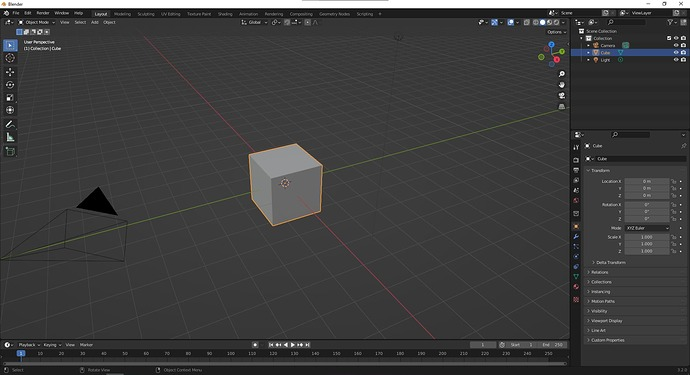
\includegraphics[width=0.8\linewidth]{blender.jpeg}
\caption{\label{fig:blender}Billede af 3D modellerings programmer blender.}
\end{figure}

I dette projekt har jeg lavet en simpel 3D engine i python med pygame biblioteket. 
Man kan se det endlige program \texttt{sigma()} på figur \ref{fig:program}.

\begin{figure}[H]
\centering
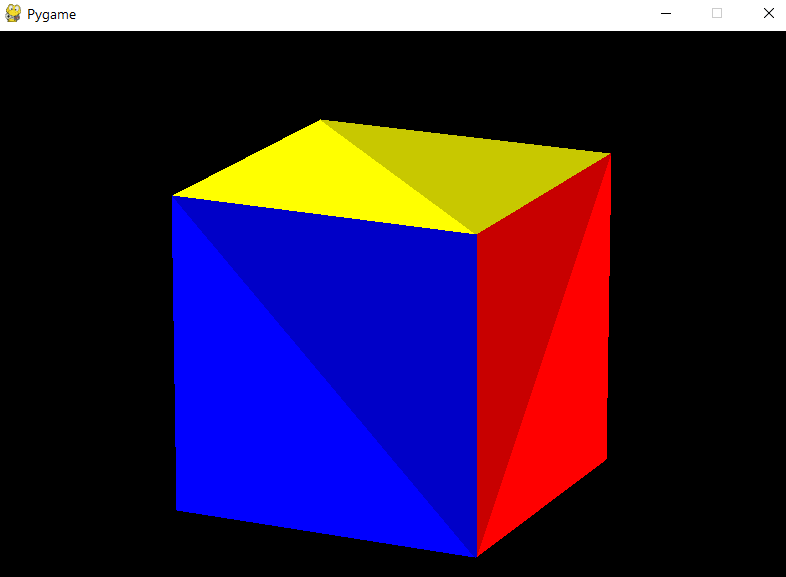
\includegraphics[width=0.7\linewidth]{program.png}
\caption{\label{fig:program}Billede af mit program.}
\end{figure}

\section{3D projektion}
3D projektion er en metode til at vise 3D objekter på en 2D skærm. 
Der findes mange forskellige metoder til at lave 3D projektion.
Se figur \ref{fig:3dpro} for en Illustration af de forskellige 3D projektion.

\begin{figure}[H]
\centering
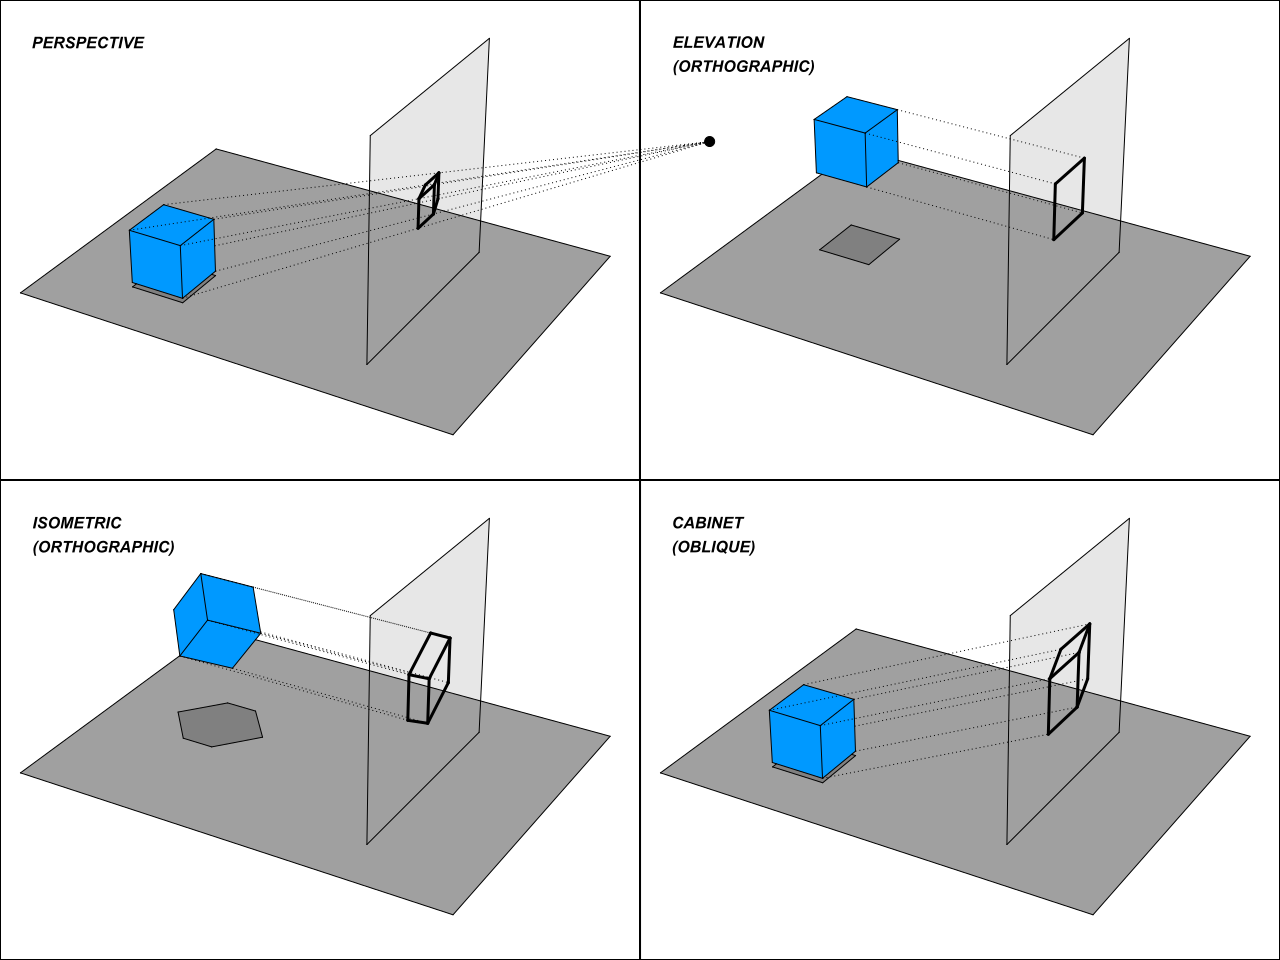
\includegraphics[width=0.7\linewidth]{3dpro.png}
\caption{\label{fig:3dpro}Illustration af de forskellige 3D projektion fra wikipedia.org.}
\end{figure}

Den som jeg har valgt at bruge er den som hedder perspective projection.
Perspective projection fungere ved at man har et punkt i 3D rummet, som kan forstårs som et kamera.
Der er en plan, som kan forstårs som en skærm.
Og så er der et punkt i 3D rummet, som er en del at et objekt.
Man kan så tegne en linje fra kameraet til punktet på objektet, og så finde ud af hvor den skærer skærmen.
Der vil man så tegne punktet på skærmen.

På figur \ref{fig:plan} kan man se perspective projection oppe fra som 2D.
Der er et punkt, som hedder $Kamera$ som er kameraet. 
Der er en plan, som er den sorte linje, det er skærmen.
Der er et punkt, som hedder $p_{c}$ som er et punkt på objektet, og i dette tilfælle er en firekant.
Man kan se at der er en linje fra kameraet til punktet $p_{c}$.
Der hvor linjen skærer skærmen, der er punktet $p_{s}$.
Det er sådan metoden fungere.

\begin{figure}[H]
\centering
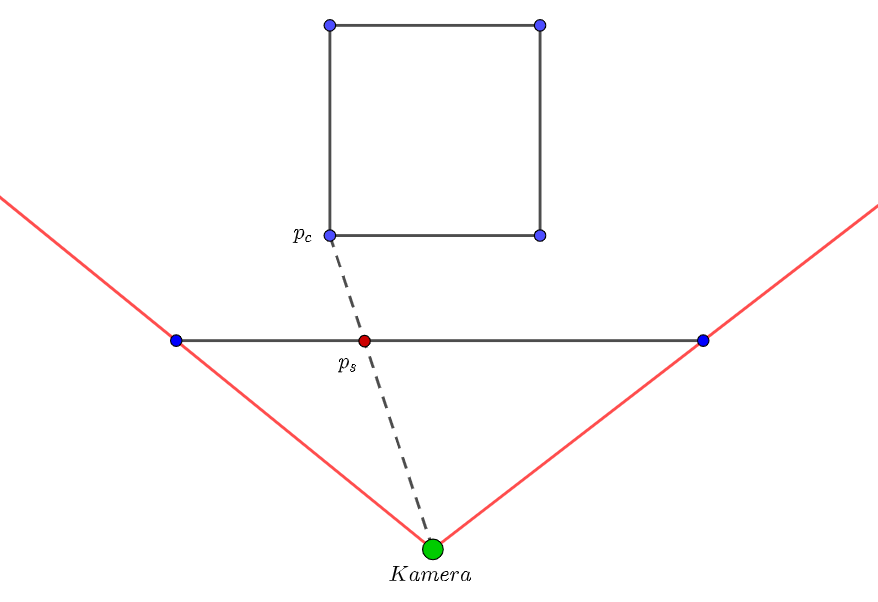
\includegraphics[width=0.7\linewidth]{plan.png}
\caption{\label{fig:plan}Illustration af 3D perspective projection set oppe fra som 2D.}
\end{figure}

\section{Pygame}
Pygame er et bibliotek til python, som gør det muligt at lave grafiske applikationer såsom spil.
Pygame laver et popup vindue, og man tenge figurer og billeder i vinduet.
Pygame har noget som hedder et game loop. Et game loop er et loop som opdaterer progammet hele tiden.
Den start med at først håndterer input fx. tastatur eller mus.
Så opdaterer spillets tilstand og logikken fx. bevægelse af objekter.
Og til sidst tegner det objekterne på skærmen.
Et meget simpelt game loop kan ses i koden på figur \ref{fig:pgkode}.

\begin{figure}[H]
\begin{minted}[xleftmargin=20pt,linenos]{python}
import pygame
import sys

pygame.init()
screenWidth = 800
screenHeight = 600
black = (0, 0, 0)

screen = pygame.display.set_mode((screenWidth, screenHeight))
pygame.display.set_caption("Pygame")
clock = pygame.time.Clock()
FPS = 60
# game loop
running = True
while running:
    clock.tick(FPS)
    # inputs
    for event in pygame.event.get():
        if event.type == pygame.QUIT:
            running = False
        elif event.type == pygame.KEYDOWN:
            if event.key == pygame.K_ESCAPE:
                running = False
    # updates

    # draw
    screen.fill(black)
    pygame.display.flip()
\end{minted}
\caption{\label{fig:pgkode}Kode for meget simpelt game loop.}
\end{figure}

\section{3D punkt til 2D punkt}
For at kunne være i stand til at tegne 3D objekter, på en 2D skærm, 
startet jeg med at lave en funktion som hedder \texttt{getPointOnPlan}.
\texttt{getPointOnPlan} tager 3 argumenter.
Det første argument \texttt{fig} er en list af 3D punkt. (Et 3D punkt er en list med 3 floats)
Det andet argument \texttt{plan} er en list som beskriver ligningen for en plan på denne både måde: 
\texttt{[a, b, c, k]}, hvor plansligning ser sådan ud $ax+by+cz+k=0$.
Det sidste argument \texttt{pov} er et 3D punkt som beskriver kameraet.
Funktionen \texttt{getPointOnPlan} returnere en liste punkter på planen som 2D punkter. (Et 2D punkt er en list med 2 floats)
Koden kan ses i figur \ref{fig:getPointOnPlan}.

\begin{figure}[H]
\begin{minted}[xleftmargin=20pt,linenos]{python}
def getPointOnPlan(fig,plan,pov):
    final = []
    for i in range(len(fig)):
        r = []
        for j in range(len(fig[i])):
            r.append(fig[i][j]-pov[j])
        x = [pov[0],r[0]]
        y = [pov[1],r[1]]
        z = [pov[2],r[2]]
        ligning_num = plan[0]*x[0] + plan[1]*y[0] + plan[2]*z[0] + plan[3]
        ligning_t = plan[0]*x[1] + plan[1]*y[1] + plan[2]*z[1]
        t = (-(ligning_num))/ligning_t
        final.append([y[0]+t*y[1], z[0]+t*z[1]])
    return final
\end{minted}
\caption{\label{fig:getPointOnPlan}Kode for meget simpelt game loop.}
\end{figure}

For at ikke at gå for meget i dybden med matematikken, så vil jeg gå lidt overfladisk om det.
På linje 3 laver jeg et for loop som går igennem alle punkter i listen \texttt{fig}, så et punkt er \texttt{fig[i]}.
Derefter på linje 4, 5 og 6 laver jeg en retningsvektor \texttt{r} fra \texttt{pov} til \texttt{fig[i]} for at lave en linje mellem dem.
Så på linje 7, 8 og 9 opsætter jeg en liste \texttt{x}, \texttt{y} og \texttt{z} som er \texttt{pov[0]} og \texttt{r[0]} for at løse en ligning mellem planen og og linjen.
Bageefter på linje 10, 11 og 12 løser jeg en ligning for $t$. Det er hvor langt henne linjen skærer planen.
Til sidst på linje 13 tilføjer jeg $y$ og $z$ koordinaterne til listen \texttt{final} som er en liste af 2D punkter.


\section{Polygoner}


\section{Painters algorithm}

\section{Egen algorithmme}

\section{Kasser}

\section{Konklusion}

\end{document}